\section{Структура индексов в MySQL InnoDB}

В СУБД MySQL (InnoDB) используются Btree индексы, основанные на структуре данных B+tree Рисунок \ref{img:btree-structure}.

\begin{figure}[H]
  \centering
  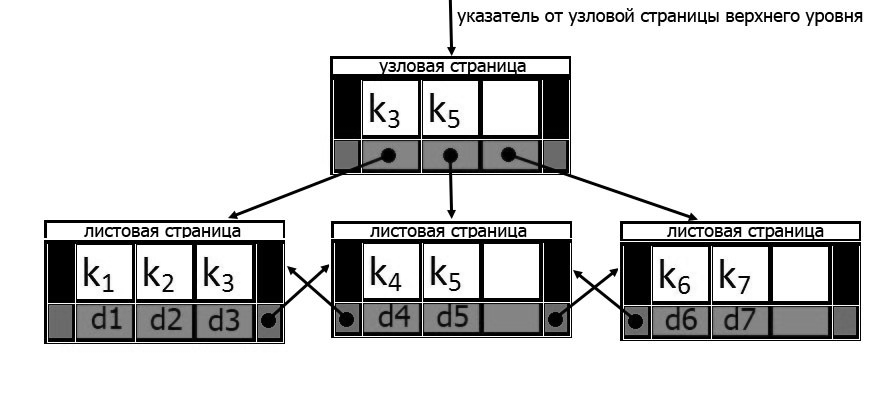
\includegraphics[scale=0.5]{btree.png}
  \caption{Структура данных B+tree.}
  \label{img:btree-structure}
\end{figure}

Где
$k_i$ - ключи ($k_i < k_i + 1$),
$d_i$ - данные.

Сложность поиска в линейной структуре данных $O(N)$, а в B+tree - $log(K)+N_k$, где $k$ — количество уровней, а $N_k$ — количество элементов в узле. Поэтому индексы, использующие структуру данных B+tree, эффективны для поиска данных. Для оптимизации поиска по диапазону в листовых страницах есть указатели на следующую и предыдущую листовую страницу.

В InnoDB данные хранятся в структуре B+tree, где в узловых страницах хранятся первичные ключи, а в листовых страницах хранятся данные. Такое дерево называется \textbf{кластерным индексом}. Над таблицей можно построить только один кластерный индекс, поскольку невозможно хранить одну и ту же запись одновременно в двух местах. Однако часть записи можно хранить в нескольких местах, что будет использоваться в покрывающих индексах, являющимися вторичными индексами.

Для оптимизации конкретных запросов используются \textbf{вторичные индексы} (далее просто индексы). В узловых страницах индексов хранятся поля, по которым создан этот индекс, а в листовых страницах хранится значение первичного ключа. Для каждой таблицы в одном запросе используется только один индекс. При использовании в запросах индекса, сначала будет найдено значение первичного ключа, затем по этому значению будут найдены данные в кластерном индексе.